\chapter{Disoluciones tampón y diagramas de predominio}\label{ch:g12:buffers-predominance}

Un análisis de sangre indica el \omterm{def:g9:acids-bases-ph:ph}{pH} de la sangre arterial: normalmente,
entre 7.38 y 7.42. Los músculos en actividad vierten ácidos en la
sangre, los pulmones expulsan de ella dióxido de carbono, los alimentos
aportan ácidos y bases; y, sin embargo, el \omterm{def:g9:acids-bases-ph:ph}{pH} apenas se mueve. Un par de
especies, un ácido y su propia base, amortigua estos golpes. Este
capítulo muestra qué forma de un par domina a un \omterm{def:g9:acids-bases-ph:ph}{pH} dado, cómo unas
gotas de un par coloreado revelan el \omterm{def:g9:acids-bases-ph:ph}{pH} y cómo una \omterm{def:g6:pure-substances-and-mixtures:mixture}{mezcla} de un ácido y
su base mantiene el \omterm{def:g9:acids-bases-ph:ph}{pH} estable.

\begin{recall}
Los \omterm{def:g12:ka-and-pka:bronsted}{pares ácido--base}, $K_a$ y $pK_a$; el \omterm{def:g9:acids-bases-ph:ph}{pH} de una disolución
(\cref{ch:g12:ka-and-pka}, \cref{ch:g9:acids-bases-ph}).
\end{recall}

\begin{omfigure}
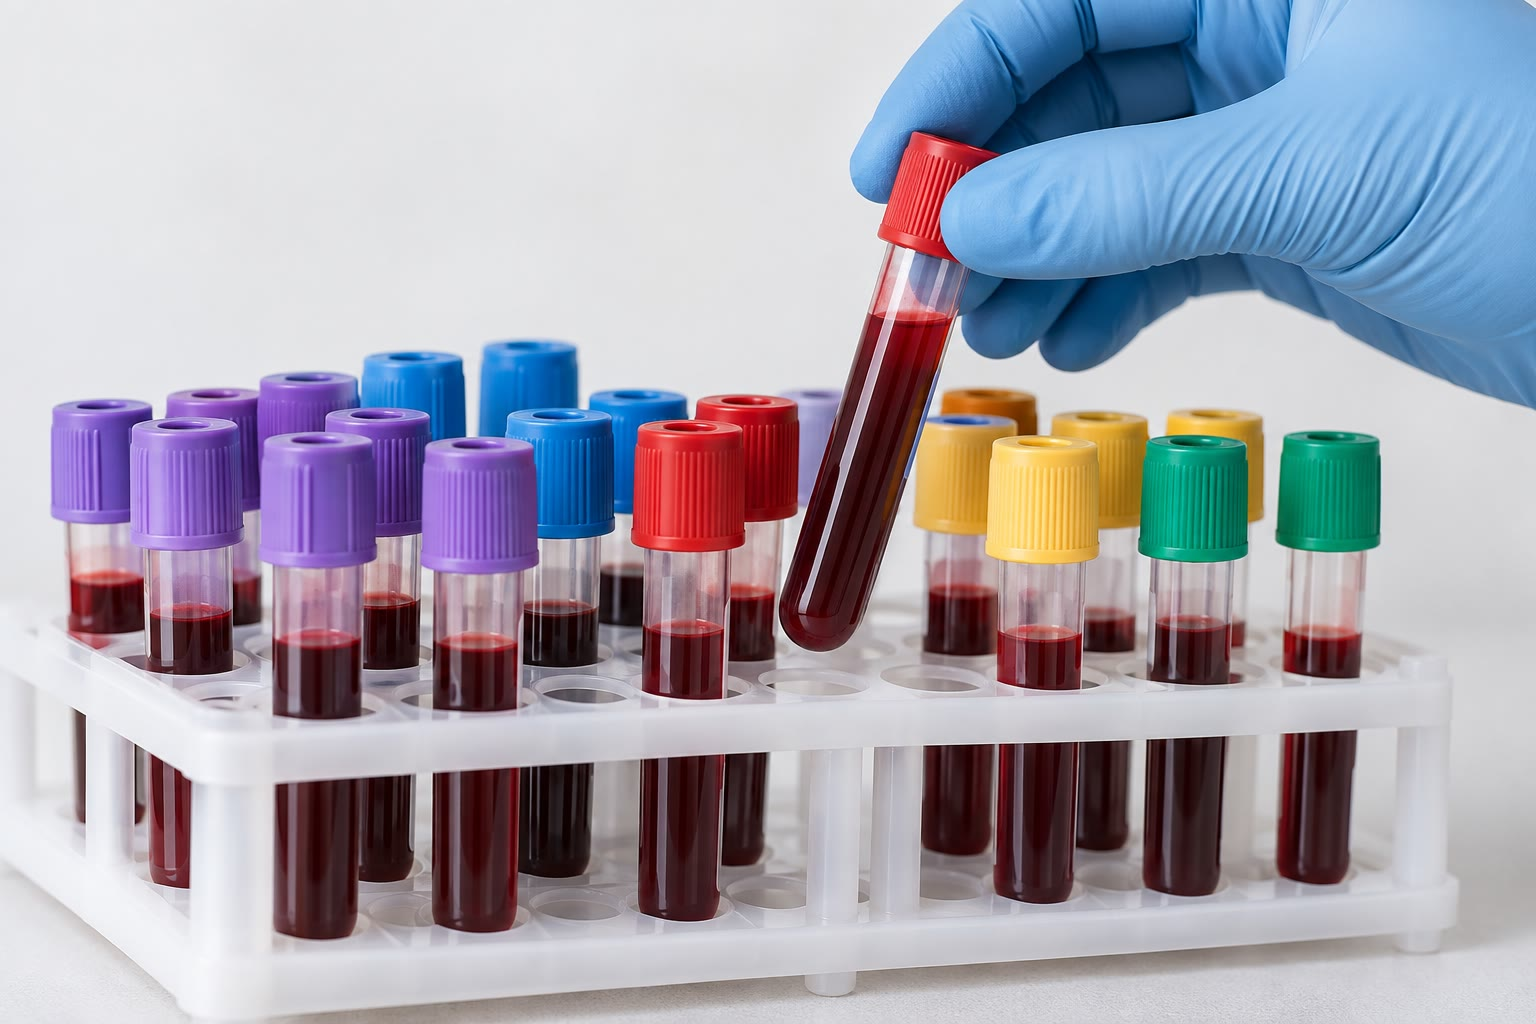
\includegraphics[width=0.45\linewidth]{images/book1/ai/g12-blood-tubes.jpg}

{\small Muestras de sangre: su \omterm{def:g9:acids-bases-ph:ph}{pH} se mantiene en un intervalo estrecho.}
\end{omfigure}

\section{Diagramas de predominio}

\begin{proposition}[Relación de Henderson]\label{prop:g12:buffers-predominance:henderson}
En cualquier \omterm{def:g6:solutions-and-solubility:solute}{disolución acuosa} que contenga el par \ce{HA}/\ce{A-},
\[
  \mathrm{pH} = pK_a + \log\frac{[\ce{A-}]}{[\ce{HA}]} .
\]
\end{proposition}

\begin{proof}
A partir de $K_a = \dfrac{[\ce{A-}][\ce{H3O+}]}{[\ce{HA}]c^\circ}$, se
toma $-\log$ en ambos miembros: $pK_a = \mathrm{pH} - \log\dfrac{[\ce{A-}]}{[\ce{HA}]}$.
\end{proof}

\begin{definition}[Diagramas de predominio y de distribución]\label{def:g12:buffers-predominance:predominance}
El \emph{diagrama de predominio}\index{diagrama de predominio} de un par
es un eje de \omterm{def:g9:acids-bases-ph:ph}{pH} dividido en el $pK_a$: por debajo predomina el ácido HA
($[\ce{HA}] > [\ce{A-}]$); por encima, la base \ce{A-}. El \emph{diagrama
de distribución}\index{diagrama de distribucion@diagrama de distribución} muestra la fracción de
cada forma, $[\ce{HA}]/c$ y $[\ce{A-}]/c$, en función del \omterm{def:g9:acids-bases-ph:ph}{pH}; las dos
curvas se cortan en $\mathrm{pH} = pK_a$.
\end{definition}

\begin{method}[Dibujar un diagrama de predominio]\label{met:g12:buffers-predominance:diagram}
\begin{enumerate}
  \item Dibuja un eje de \omterm{def:g9:acids-bases-ph:ph}{pH} de 0 a 14 y marca el $pK_a$ del par.
  \item Escribe el ácido a la izquierda del $pK_a$ y la base a la derecha.
  \item Para una especie con varios pares (un ácido con dos hidrógenos que
        ceder, un aminoácido), marca todos los $pK_a$: cada intervalo
        corresponde a una forma.
  \item A una unidad del $pK_a$, la razón ya es de 10 a 1: la forma
        minoritaria está por debajo del \qty{10}{\percent}.
\end{enumerate}
\end{method}

\begin{omfigure}
\begin{tikzpicture}[font=\small, x=0.62cm]
  % ledger: pka:ethanoic, pka:methanoic, kb:NH3, ka:H2CO3
  \foreach \y/\pk/\acid/\base in {0/3.74/{\ce{HCOOH}}/{\ce{HCOO-}},
      -1.0/4.76/{\ce{CH3COOH}}/{\ce{CH3COO-}}, -2.0/6.37/{\ce{CO2,H2O}}/{\ce{HCO3-}},
      -3.0/9.26/{\ce{NH4+}}/{\ce{NH3}}} {
    \fill[omThm!20] (0,\y) rectangle (\pk,\y+0.5);
    \fill[omDef!20] (\pk,\y) rectangle (14,\y+0.5);
    \draw[black!50] (0,\y) rectangle (14,\y+0.5);
    \node at (\pk/2,\y+0.25) {\acid};
    \node at ({(\pk+14)/2},\y+0.25) {\base};
    \draw[thick] (\pk,\y-0.08) -- (\pk,\y+0.58);
    \node[font=\scriptsize, anchor=south] at (\pk,\y+0.55) {\pk};
  }
  \draw[->] (0,-3.4) -- (14.5,-3.4) node[right] {pH};
  \foreach \k in {0,2,4,6,8,10,12,14} \draw (\k,-3.35) -- (\k,-3.45) node[below, font=\scriptsize] {\k};
\end{tikzpicture}

{\small \omterm{def:g12:buffers-predominance:predominance}{Diagramas de predominio} de cuatro pares: el ácido (a la
izquierda, en rojo) domina por debajo de su $pK_a$; la base (a la
derecha, en azul), por encima.}
\end{omfigure}

\begin{omfigure}
\begin{minipage}{0.49\linewidth}
\begin{tikzpicture}
\begin{axis}[width=\linewidth, height=5cm, xmin=0, xmax=14, ymin=0, ymax=1.05,
    xlabel={pH}, ylabel={fracción}, axis lines*=left, ymajorgrids,
    grid style={gray!20}, tick label style={font=\scriptsize},
    label style={font=\small}, title={\small ácido etanoico},
    title style={yshift=-4pt}]
  \addplot[very thick, omThm] table[x=pH, y=HA] {figdata/out/grade-12-buffers-predominance-a.dat};
  \addplot[very thick, omDef] table[x=pH, y=A] {figdata/out/grade-12-buffers-predominance-a.dat};
  \addplot[dashed, black!50] coordinates {(4.76,0) (4.76,1)};
  \node[font=\scriptsize, omThm] at (axis cs:2.2,0.85) {\ce{CH3COOH}};
  \node[font=\scriptsize, omDef] at (axis cs:7.6,0.85) {\ce{CH3COO-}};
\end{axis}
\end{tikzpicture}
\end{minipage}\hfill
\begin{minipage}{0.49\linewidth}
\begin{tikzpicture}
\begin{axis}[width=\linewidth, height=5cm, xmin=0, xmax=14, ymin=0, ymax=1.05,
    xlabel={pH}, ylabel={fracción}, axis lines*=left, ymajorgrids,
    grid style={gray!20}, tick label style={font=\scriptsize},
    label style={font=\small}, title={\small glicina},
    title style={yshift=-4pt}]
  \addplot[very thick, omThm] table[x=pH, y=cation] {figdata/out/grade-12-buffers-predominance-b.dat};
  \addplot[very thick, omMeth] table[x=pH, y=zwitterion] {figdata/out/grade-12-buffers-predominance-b.dat};
  \addplot[very thick, omDef] table[x=pH, y=anion] {figdata/out/grade-12-buffers-predominance-b.dat};
  \node[font=\scriptsize, omThm] at (axis cs:1.0,0.55) {catión};
  \node[font=\scriptsize, omMeth] at (axis cs:6.1,0.88) {zwitterión};
  \node[font=\scriptsize, omDef] at (axis cs:12.6,0.55) {anión};
\end{axis}
\end{tikzpicture}
\end{minipage}

{\small \omterm{def:g12:buffers-predominance:predominance}{Diagramas de distribución}, calculados a partir de los valores de
$pK_a$. Izquierda: ácido etanoico; las curvas se cortan en 4.76.
Derecha: glicina, \ce{H2N-CH2-COOH}, con dos pares ($pK_a$ 2.35 y 9.78):
el \omterm{def:g9:ions:ion}{catión} \ce{H3N+-CH2-COOH}, el zwitterión \ce{H3N+-CH2-COO-} y el \omterm{def:g9:ions:ion}{anión}
\ce{H2N-CH2-COO-}.}
\end{omfigure}

\begin{example}[La glicina en el cuerpo]\label{ex:g12:buffers-predominance:glycine}
% ledger: pka:glycine1, pka:glycine2, ph:blood
Al \omterm{def:g9:acids-bases-ph:ph}{pH} de la sangre, alrededor de 7.4, la glicina está entre sus dos
valores de $pK_a$: se encuentra casi por completo en forma de
zwitterión, con una carga positiva en el nitrógeno y una carga negativa
en el carboxilato, neutra en conjunto. Todos los aminoácidos se
comportan del mismo modo.
\end{example}

\section{Indicadores ácido--base}


\begin{definition}[Indicador ácido--base, zona de viraje]\label{def:g12:buffers-predominance:indicator}
Un \emph{indicador ácido--base}\index{indicador acido--base@indicador ácido--base} es un par
\ce{HInd}/\ce{Ind-} cuyas dos formas tienen colores distintos y que se
usa en cantidades muy pequeñas. Su \emph{zona de viraje}\index{zona de viraje}
es el intervalo de \omterm{def:g9:acids-bases-ph:ph}{pH} en el que se ve cambiar el color, aproximadamente
de $pK_a - 1$ a $pK_a + 1$: por debajo se ve el color de \ce{HInd}; por
encima, el de \ce{Ind-}; y entre ambos, una \omterm{def:g6:pure-substances-and-mixtures:mixture}{mezcla} de los dos.
\end{definition}

\begin{omfigure}
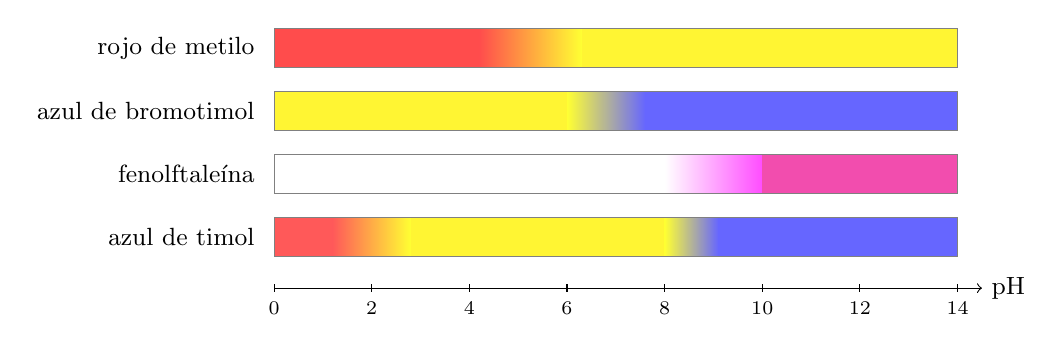
\begin{tikzpicture}[font=\small, x=0.62cm]
  % ledger: ind:methyl-red, ind:BBT, ind:phenolphthalein, ind:thymol-blue, ind:range-rule
  \foreach \y/\name/\a/\b/\ca/\cm/\cb in {
      0/{rojo de metilo}/4.2/6.3/red!70/orange/yellow!80,
      -0.8/{azul de bromotimol}/6.0/7.6/yellow!80/green!60/blue!60,
      -1.6/{fenolftaleína}/8.0/10.0/white/magenta!25/magenta!70} {
    \fill[\ca] (0,\y) rectangle (\a,\y+0.5);
    \shade[left color=\ca, right color=\cb] (\a,\y) rectangle (\b,\y+0.5);
    \fill[\cb] (\b,\y) rectangle (14,\y+0.5);
    \draw[black!50] (0,\y) rectangle (14,\y+0.5);
    \node[anchor=east] at (-0.2,\y+0.25) {\name};
  }
  \fill[red!65] (0,-2.4) rectangle (1.2,-1.9);
  \shade[left color=red!65, right color=yellow!80] (1.2,-2.4) rectangle (2.8,-1.9);
  \fill[yellow!80] (2.8,-2.4) rectangle (8.0,-1.9);
  \shade[left color=yellow!80, right color=blue!60] (8.0,-2.4) rectangle (9.1,-1.9);
  \fill[blue!60] (9.1,-2.4) rectangle (14,-1.9);
  \draw[black!50] (0,-2.4) rectangle (14,-1.9);
  \node[anchor=east] at (-0.2,-2.15) {azul de timol};
  \draw[->] (0,-2.8) -- (14.5,-2.8) node[right] {pH};
  \foreach \k in {0,2,4,6,8,10,12,14} \draw (\k,-2.75) -- (\k,-2.85) node[below, font=\scriptsize] {\k};
\end{tikzpicture}

{\small Colores de cuatro indicadores en función del \omterm{def:g9:acids-bases-ph:ph}{pH}; las partes
sombreadas son las \omterm{def:g12:buffers-predominance:indicator}{zonas de viraje}. El azul de timol, con dos pares,
tiene dos \omterm{def:g12:buffers-predominance:indicator}{zonas de viraje}.}
\end{omfigure}

\begin{method}[Elegir un indicador]\label{met:g12:buffers-predominance:indicator}
Para detectar cuándo una disolución pasa por un \omterm{def:g9:acids-bases-ph:ph}{pH} dado (el \omterm{def:g9:acids-bases-ph:ph}{pH} al final
de una \omterm{def:g11:titration:titration}{valoración}, por ejemplo), elige un indicador cuya \omterm{def:g12:buffers-predominance:indicator}{zona de viraje}
contenga ese \omterm{def:g9:acids-bases-ph:ph}{pH}: el color cambia entonces justo ahí.
\end{method}

\section{Disoluciones tampón}

\begin{definition}[Disolución tampón]\label{def:g12:buffers-predominance:buffer}
Una \emph{disolución tampón}\index{disolucion tampon@disolución tampón} es una disolución
cuyo \omterm{def:g9:acids-bases-ph:ph}{pH} varía muy poco cuando se le añade un poco de ácido o de base, o
cuando se diluye. Suele estar formada por un \omterm{def:g12:ka-and-pka:strong-acid}{ácido débil} y su base
conjugada en cantidades comparables; su \omterm{def:g9:acids-bases-ph:ph}{pH} es entonces próximo al
$pK_a$ del par.
\end{definition}

\begin{proposition}[Por qué resiste un tampón]\label{prop:g12:buffers-predominance:buffer}
En un tampón de \ce{HA} y \ce{A-}, un \omterm{def:g12:ka-and-pka:strong-acid}{ácido fuerte} añadido es consumido
por \ce{A-} (\ce{A- + H3O+ -> HA + H2O}) y una \omterm{def:g12:ka-and-pka:strong-acid}{base fuerte} añadida, por
\ce{HA} (\ce{HA + OH- -> A- + H2O}); la razón $[\ce{A-}]/[\ce{HA}]$, y
por tanto el \omterm{def:g9:acids-bases-ph:ph}{pH}, cambian solo un poco. La \omterm{def:g10:concentration-and-dilution:dilution}{dilución} no cambia en absoluto
la razón.
\end{proposition}

\begin{proof}
Por la relación de Henderson, el \omterm{def:g9:acids-bases-ph:ph}{pH} solo depende de la razón. Añadir
\qty{1}{mmol} de ácido a un tampón con \qty{10}{mmol} de cada forma
cambia la razón de $10/10$ a $9/11$, y el \omterm{def:g9:acids-bases-ph:ph}{pH} solo en
$\log(9/11) = -0.09$.
\end{proof}

\begin{omfigure}
\begin{tikzpicture}
\begin{axis}[width=0.75\linewidth, height=5.6cm, xmin=0, xmax=10, ymin=0,
    ymax=8, xlabel={\ce{HCl} a \qty{0.10}{mol/L} añadido (\si{mL})},
    ylabel={pH}, axis lines*=left, ymajorgrids, grid style={gray!20},
    tick label style={font=\small}, label style={font=\small},
    legend style={font=\small, at={(0.98,0.97)}, anchor=north east,
    draw=none, fill=white}, legend cell align=left]
  % ledger: pka:ethanoic (buffer recipe: exercise data)
  \addplot[very thick, omThm, mark=*, mark size=1.3pt] table[x=V, y=water]
    {figdata/out/grade-12-buffers-predominance-c.dat};
  \addplot[very thick, omDef, mark=*, mark size=1.3pt] table[x=V, y=buffer]
    {figdata/out/grade-12-buffers-predominance-c.dat};
  \legend{\qty{100}{mL} de agua pura, \qty{100}{mL} de tampón etanoato}
\end{axis}
\end{tikzpicture}

{\small Adición de ácido clorhídrico a agua pura y a un tampón de ácido
etanoico y etanoato de sodio (\qty{0.10}{mol/L} de cada uno). El \omterm{def:g9:acids-bases-ph:ph}{pH} del
agua baja de 7 a alrededor de 2; el del tampón, de 4.76 a 4.67.}
\end{omfigure}

\begin{method}[Preparar un tampón]\label{met:g12:buffers-predominance:prepare}
\begin{enumerate}
  \item Elige un par cuyo $pK_a$ esté a menos de una unidad del \omterm{def:g9:acids-bases-ph:ph}{pH}
        deseado (idealmente, muy cerca).
  \item Calcula la razón $[\ce{A-}]/[\ce{HA}] = 10^{\mathrm{pH} - pK_a}$.
  \item \omterm{def:g6:pure-substances-and-mixtures:mixture}{Mezcla} el \omterm{def:g12:ka-and-pka:strong-acid}{ácido débil} y una sal de su base en esa razón, a
        concentraciones lo bastante altas para absorber las cantidades de
        ácido o de base.
\end{enumerate}
\end{method}

\begin{inthelab}[Preparar un tampón de pH 4.8]
Se \omterm{def:g2:mixing-and-dissolving:mix}{mezclan} \qty{50.0}{mL} de ácido etanoico a \qty{0.10}{mol/L} con
\qty{50.0}{mL} de etanoato de sodio a \qty{0.10}{mol/L}; un \omterm{def:g9:acids-bases-ph:ph-paper}{pHmetro}
marca alrededor de 4.8. Unas gotas de ácido clorhídrico a
\qty{1}{mol/L} apenas mueven la lectura, mientras que las mismas gotas en
\qty{100}{mL} de agua destilada la bajan a alrededor de 3.
\end{inthelab}

\section{Los tampones en los seres vivos}

\begin{example}[El tampón de la sangre]\label{ex:g12:buffers-predominance:blood}
% ledger: pk:blood-bicarb, ph:blood, hco3:blood
El principal tampón de la sangre es el par formado por el dióxido de
carbono disuelto y el \omterm{def:g9:ions:ion}{ion} hidrogenocarbonato, \ce{CO2,H2O}/\ce{HCO3-}.
En la sangre, los fisiólogos usan para él la relación $\mathrm{pH} = 6.1 +
\log\big([\ce{HCO3-}]/[\ce{CO2}]\big)$. Los pulmones eliminan el dióxido
de carbono y los riñones ajustan el hidrogenocarbonato: juntos mantienen
la razón y, por tanto, el \omterm{def:g9:acids-bases-ph:ph}{pH}.
\end{example}

\begin{omfigure}
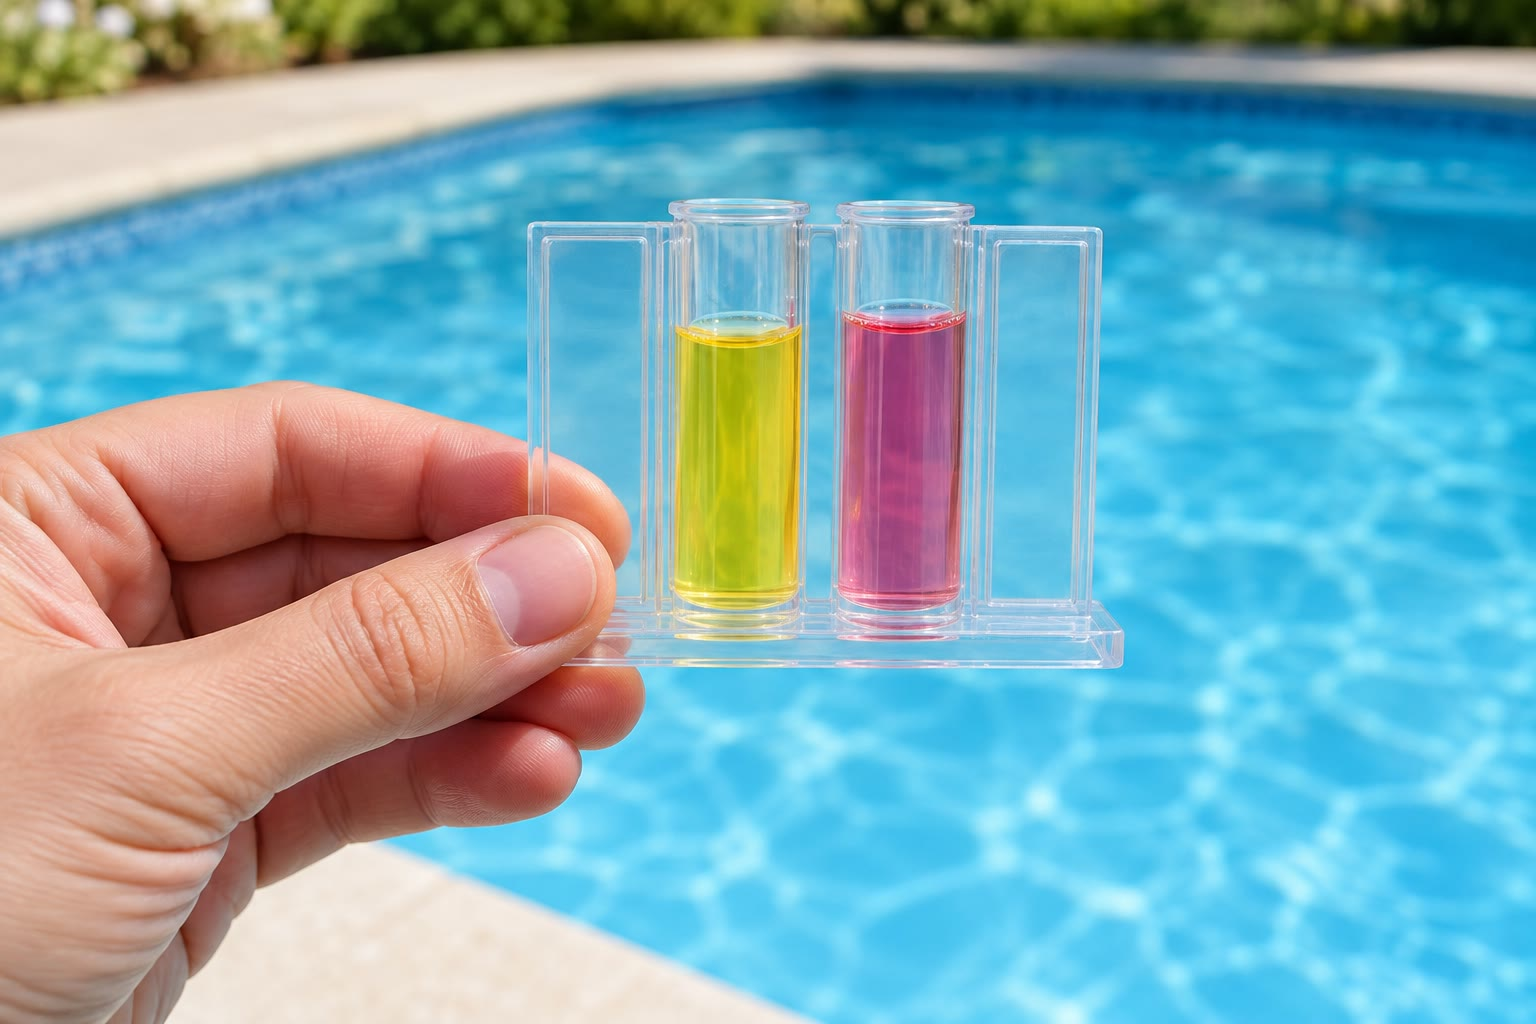
\includegraphics[width=0.45\linewidth]{images/book1/ai/g12-pool-test.jpg}

{\small Análisis del agua de una piscina: los colores de los indicadores
dan el \omterm{def:g9:acids-bases-ph:ph}{pH}.}
\end{omfigure}

\section{Ejercicios}


\begin{exercise}[$\star$]\label{exo:g12:buffers-predominance:1}
¿Qué forma del par \ce{CH3COOH}/\ce{CH3COO-} ($pK_a = 4.76$) predomina a
\omterm{def:g9:acids-bases-ph:ph}{pH} 2, a \omterm{def:g9:acids-bases-ph:ph}{pH} 4.76 y a \omterm{def:g9:acids-bases-ph:ph}{pH} 7?
\end{exercise}

\begin{exercise}[$\star$]\label{exo:g12:buffers-predominance:2}
En el \omterm{def:g12:buffers-predominance:predominance}{diagrama de distribución} del ácido etanoico, lee la fracción de
\ce{CH3COO-} a \omterm{def:g9:acids-bases-ph:ph}{pH} 4 y a \omterm{def:g9:acids-bases-ph:ph}{pH} 6.
\end{exercise}

\begin{exercise}[$\star$]\label{exo:g12:buffers-predominance:3}
¿Qué color muestra el azul de bromotimol a \omterm{def:g9:acids-bases-ph:ph}{pH} 5? ¿Y a \omterm{def:g9:acids-bases-ph:ph}{pH} 7? ¿Y a \omterm{def:g9:acids-bases-ph:ph}{pH} 9?
\end{exercise}

\begin{exercise}[$\star$]\label{exo:g12:buffers-predominance:4}
¿Qué forma del par \ce{NH4+}/\ce{NH3} predomina en una disolución a
\omterm{def:g9:acids-bases-ph:ph}{pH} 7.4? ¿Y a \omterm{def:g9:acids-bases-ph:ph}{pH} 11?
\end{exercise}

\begin{exercise}[$\star$]\label{exo:g12:buffers-predominance:5}
¿Por qué los indicadores se usan en cantidades muy pequeñas?
\end{exercise}

\begin{exercise}[$\star\star$]\label{exo:g12:buffers-predominance:6}
Calcula la razón $[\ce{CH3COO-}]/[\ce{CH3COOH}]$ a \omterm{def:g9:acids-bases-ph:ph}{pH} 3.76, 4.76 y 5.76.
\end{exercise}

\begin{exercise}[$\star\star$]\label{exo:g12:buffers-predominance:7}
Una \omterm{def:g11:titration:titration}{valoración} termina a \omterm{def:g9:acids-bases-ph:ph}{pH} 8.7. ¿Cuál de los cuatro indicadores de la
figura elegirías? ¿Por qué no el rojo de metilo?
\end{exercise}

\begin{exercise}[$\star\star$]\label{exo:g12:buffers-predominance:8}
Un tampón contiene \qty{0.20}{mol/L} de ácido etanoico y
\qty{0.10}{mol/L} de etanoato de sodio. Calcula su \omterm{def:g9:acids-bases-ph:ph}{pH}.
\end{exercise}

\begin{exercise}[$\star\star$]\label{exo:g12:buffers-predominance:9}
Con el diagrama de la glicina, da la forma predominante a \omterm{def:g9:acids-bases-ph:ph}{pH} 1, 6 y 12,
con su carga.
\end{exercise}

\begin{exercise}[$\star\star$]\label{exo:g12:buffers-predominance:10}
Lee las curvas de respuesta: ¿cuánto baja el \omterm{def:g9:acids-bases-ph:ph}{pH} del agua tras añadir
\qty{1.0}{mL} de ácido? ¿Y el del tampón?
\end{exercise}

\begin{exercise}[$\star\star$]\label{exo:g12:buffers-predominance:11}
¿Qué par de la figura de predominio elegirías para preparar un tampón de
\omterm{def:g9:acids-bases-ph:ph}{pH} 9.5? ¿En qué razón mezclarías sus dos formas?
\end{exercise}

\begin{exercise}[$\star\star\star$]\label{exo:g12:buffers-predominance:12}
El tampón etanoato de la figura (\qty{10}{mmol} de cada forma) recibe
ácido clorhídrico. ¿Cuánto ácido puede admitir antes de que su \omterm{def:g9:acids-bases-ph:ph}{pH} haya
bajado una unidad? ¿Por qué se dice que un tampón más concentrado tiene
una capacidad mayor?
\end{exercise}

\begin{exercise}[$\star\star\star$]\label{exo:g12:buffers-predominance:13}
¿Qué volumen de disolución de etanoato de sodio a \qty{0.10}{mol/L} hay
que añadir a \qty{100}{mL} de ácido etanoico a \qty{0.10}{mol/L} para
obtener un tampón de \omterm{def:g9:acids-bases-ph:ph}{pH} 5.0?
\end{exercise}

\begin{exercise}[$\star\star\star$]\label{exo:g12:buffers-predominance:14}
El azul de timol tiene dos \omterm{def:g12:buffers-predominance:indicator}{zonas de viraje}. Explica por qué y da su color
a \omterm{def:g9:acids-bases-ph:ph}{pH} 1, 5 y 10.
\end{exercise}

\begin{exercise}[$\star\star\star$]\label{exo:g12:buffers-predominance:15}
Un tampón de \omterm{def:g9:acids-bases-ph:ph}{pH} 4.76 se diluye diez veces con agua destilada. ¿Cuál es su
nuevo \omterm{def:g9:acids-bases-ph:ph}{pH}, según la relación de Henderson? ¿Qué ocurre si se diluye diez
veces un \omterm{def:g12:ka-and-pka:strong-acid}{ácido fuerte} del mismo \omterm{def:g9:acids-bases-ph:ph}{pH}?
\end{exercise}

\section{Problema: el tampón de la sangre}

\begin{problem}[{Problema de fin de semana --- ¿qué razón entre hidrogenocarbonato y
dióxido de carbono mantiene la sangre a pH 7.4?}]
\label{pb:g12:buffers-predominance:1}
% ledger: pk:blood-bicarb, ph:blood, hco3:blood
El \omterm{def:g9:acids-bases-ph:ph}{pH} de la sangre arterial está normalmente entre 7.38 y 7.42. Su
principal tampón es el par \ce{CO2,H2O}/\ce{HCO3-}, para el que los
fisiólogos usan $\mathrm{pH} = 6.1 + \log\big([\ce{HCO3-}]/[\ce{CO2}]\big)$.
La concentración normal de hidrogenocarbonato en la sangre es de 22 a
\qty{28}{mmol/L}.

\medskip
\noindent\textbf{Parte I --- El par.}
\begin{enumerate}
  \item Escribe la reacción del dióxido de carbono disuelto con el agua
        que da \omterm{def:g9:ions:ion}{iones} hidrogenocarbonato.
  \item ¿Qué especie es el ácido y cuál la base?
  \item El valor 6.1 difiere del 6.37 de la tabla de $pK_a$. Da una razón
        (piensa en la temperatura del cuerpo y en los demás \omterm{def:g9:ions:ion}{iones}
        presentes).
  \item ¿Qué cantidad de hidrogenocarbonato contienen \qty{5.0}{L} de
        sangre a \qty{24}{mmol/L}?
\end{enumerate}

\medskip
\noindent\textbf{Parte II --- Predominio.}
\begin{enumerate}[resume]
  \item Dibuja el \omterm{def:g12:buffers-predominance:predominance}{diagrama de predominio} del par con $pK = 6.1$.
  \item ¿Qué forma predomina en la sangre?
  \item ¿Es la sangre ligeramente ácida o ligeramente básica?
\end{enumerate}

\medskip
\noindent\textbf{Parte III --- La razón.}
\begin{enumerate}[resume]
  \item Con la relación, calcula la razón $[\ce{HCO3-}]/[\ce{CO2}]$ a
        \omterm{def:g9:acids-bases-ph:ph}{pH} 7.4.
  \item Con $[\ce{HCO3-}] = \qty{24}{mmol/L}$, calcula $[\ce{CO2}]$.
  \item Calcula la razón en los dos extremos del intervalo normal, 7.38 y
        7.42.
  \item ¿Qué fracción del par está en forma de hidrogenocarbonato a
        \omterm{def:g9:acids-bases-ph:ph}{pH} 7.4?
  \item Una sangre demasiado básica puede llegar a \omterm{def:g9:acids-bases-ph:ph}{pH} 7.6. ¿Cuál es
        entonces la razón?
\end{enumerate}

\medskip
\noindent\textbf{Parte IV --- Cuando se pierde el equilibrio.}
\begin{enumerate}[resume]
  \item Durante un esfuerzo intenso entran ácidos en la sangre. ¿Qué
        forma del par los consume? Escribe la reacción.
  \item Si el \omterm{def:g9:acids-bases-ph:ph}{pH} bajara a 7.1, ¿en qué se convertiría la razón?
  \item Con el hidrogenocarbonato sin cambios, ¿cuánto tendría que
        aumentar el dióxido de carbono? ¿Qué hacen los pulmones para
        contrarrestarlo?
  \item ¿Por qué un \omterm{def:g12:ka-and-pka:strong-acid}{ácido débil} con su base, y no un \omterm{def:g12:ka-and-pka:strong-acid}{ácido fuerte}, es la
        herramienta adecuada para mantener un \omterm{def:g9:acids-bases-ph:ph}{pH}?
  \item ¿Cuánto cambia el \omterm{def:g9:acids-bases-ph:ph}{pH} si las dos concentraciones se dividen por
        dos? ¿Por qué?
  \item Da la respuesta final: ¿cuál es la razón entre hidrogenocarbonato
        y dióxido de carbono en la sangre a \omterm{def:g9:acids-bases-ph:ph}{pH} 7.4?
\end{enumerate}
\end{problem}
